\documentclass[compress]{beamer} 
\usepackage{amsmath}
\usepackage{amsfonts}
\usepackage{graphicx}
%\usepackage{epstopdf}
\usepackage{hyperref}
\usepackage{multirow}
\usepackage{verbatim}
%\usepackage[small,compact]{titlesec} 
%\usecolortheme{beaver}
\usetheme{Hannover}
%\usecolortheme{whale}

%\usepackage{pxfonts}
%\usepackage{isomath}
%\usepackage{mathpazo}
%\usepackage{arev} %     (Arev/Vera Sans)
%\usepackage{eulervm} %_   (Euler Math)
%\usepackage{fixmath} %  (Computer Modern)
%\usepackage{hvmath} %_   (HV-Math/Helvetica)
%\usepackage{tmmath} %_   (TM-Math/Times)
%\usepackage{tgheros}
%\usepackage{cmbright}
%\usepackage{ccfonts} \usepackage[T1]{fontenc}
%\usepackage[garamond]{mathdesign}
\usepackage{color}
\usepackage{ulem}

\setbeamertemplate{navigation symbols}{}
\AtBeginSection[] % Do nothing for \section*
{ \frame{\sectionpage} }

\newcommand{\argmax}{\operatornamewithlimits{arg\,max}}
\newcommand{\argmin}{\operatornamewithlimits{arg\,min}}
\def\inprobLOW{\rightarrow_p}
\def\inprobHIGH{\,{\buildrel p \over \rightarrow}\,} 
\def\inprob{\,{\inprobHIGH}\,} 
\def\indist{\,{\buildrel d \over \rightarrow}\,} 
\def\F{\mathbb{F}}
\def\R{\mathbb{R}}
\newcommand{\gmatrix}[1]{\begin{pmatrix} {#1}_{11} & \cdots &
    {#1}_{1n} \\ \vdots & \ddots & \vdots \\ {#1}_{m1} & \cdots &
    {#1}_{mn} \end{pmatrix}}
\newcommand{\iprod}[2]{\left\langle {#1} , {#2} \right\rangle}
\newcommand{\norm}[1]{\left\Vert {#1} \right\Vert}
\newcommand{\abs}[1]{\left\vert {#1} \right\vert}
\renewcommand{\det}{\mathrm{det}}
\newcommand{\rank}{\mathrm{rank}}
\newcommand{\spn}{\mathrm{span}}
\newcommand{\row}{\mathrm{Row}}
\newcommand{\col}{\mathrm{Col}}
\renewcommand{\dim}{\mathrm{dim}}
\newcommand{\prefeq}{\succeq}
\newcommand{\pref}{\succ}
\newcommand{\seq}[1]{\{{#1}_n \}_{n=1}^\infty }
\renewcommand{\to}{{\rightarrow}}


\title{Differential Calculus}
\author{Paul Schrimpf}
\institute{UBC \\ Economics 526}
\date{\today}

\begin{document}

\frame{\titlepage}
%\setcounter{tocdepth}{2}

% \begin{frame}
%   \frametitle{Midterm}
%   \includegraphics[width=0.6\textwidth,angle=270]{midterm} \\

%   \begin{tabular}{c|ccc|ccc}
%     Question & 1 & 2 & 3 & 4 & 5 & 6 \\ \hline
%     N & 50 & 9 & 43  & 50 & 33 & 19\\
%     Average & 24 & 21 & 22 & 23 &  21 & 18 \\  \hline
%   \end{tabular}
% \end{frame}

\begin{frame}
  \tableofcontents  
\end{frame}

\section{Derivatives}

\subsection{Partial derivatives}
\begin{frame}
  \frametitle{Partial derivatives}
  \begin{definition}
    Let $f:\R^n \to R$. The $i$th \textbf{partial derivative} of $f$ is 
    \[ \frac{\partial f}{\partial x_i} (x_0) = \lim_{h \to 0}
    \frac{f(x_{01},...,x_{0i}, ... x_{0n}) - f(x_0)}{h}. \]
  \end{definition}
\end{frame}
\subsection{Examples}
\begin{frame}
\begin{example}
  Let $f:\R^n \to \R$ be a production function. Then we call
  $\frac{\partial f}{\partial x_i}$ the \textbf{marginal product} of
  $x_i$. If $f$ is Cobb-Douglas, $f(k,l) = Ak^\alpha l^\beta$, where
  $k$ is capital and $l$ is labor, then the marginal products of
  capital and labor are
  \begin{align*}
    \frac{\partial f}{\partial k} (k,l) = & A \alpha k^{\alpha-1}
    l^\beta \\
    \frac{\partial f}{\partial l} (k,l) = & A \beta k^{\alpha}
    l^{\beta -1}.
  \end{align*}
\end{example}
\end{frame}

\begin{frame}
\begin{example}
  If $u:\R^n \to \R$ is a utility function, then we call
  $\frac{\partial u}{\partial x_i}$ the marginal utility of $x_i$.  
  If $u$ is CRRA, 
  \[u(c_1,...,c_T) =
  \sum_{t=1}^T \beta^t \frac{c_t^{1-\gamma}}{1-\gamma} \]
  then  the marginal utility of consumption in period $t$ is 
  \[ \frac{\partial u}{\partial c_t} = \beta^t c_t^{-\gamma}. \]
\end{example}
\end{frame}

\begin{frame}
  \begin{example}[Demand elasticities]
    \begin{itemize}
    \item  $q_1:\R^3 \to \R$ is 
      a demand function with three arguments: own price $p_1$, the price
      of another good, $p_2$, and consumer income, $y$
    \item Own price
      elasticity 
      \[ \epsilon_{q_1,p_1} = \frac{\partial q_1}{\partial p_1}
      \frac{p_1}{q_1(p_1,p_2,y)}. \]
    \item Cross price elasticity 
      \[ \epsilon_{q_1,p_2} = \frac{\partial q_1}{\partial p_2}
      \frac{p_2}{q_1(p_1,p_2,y)}. \]
    \item Income elasticity of demand 
      \[ \epsilon_{q_1,y} = \frac{\partial q_1}{\partial y}
      \frac{y}{q_1(p_1,p_2,y)}. \]
    \end{itemize}
  \end{example}
\end{frame}

\subsection{Total derivatives}

\begin{frame}
  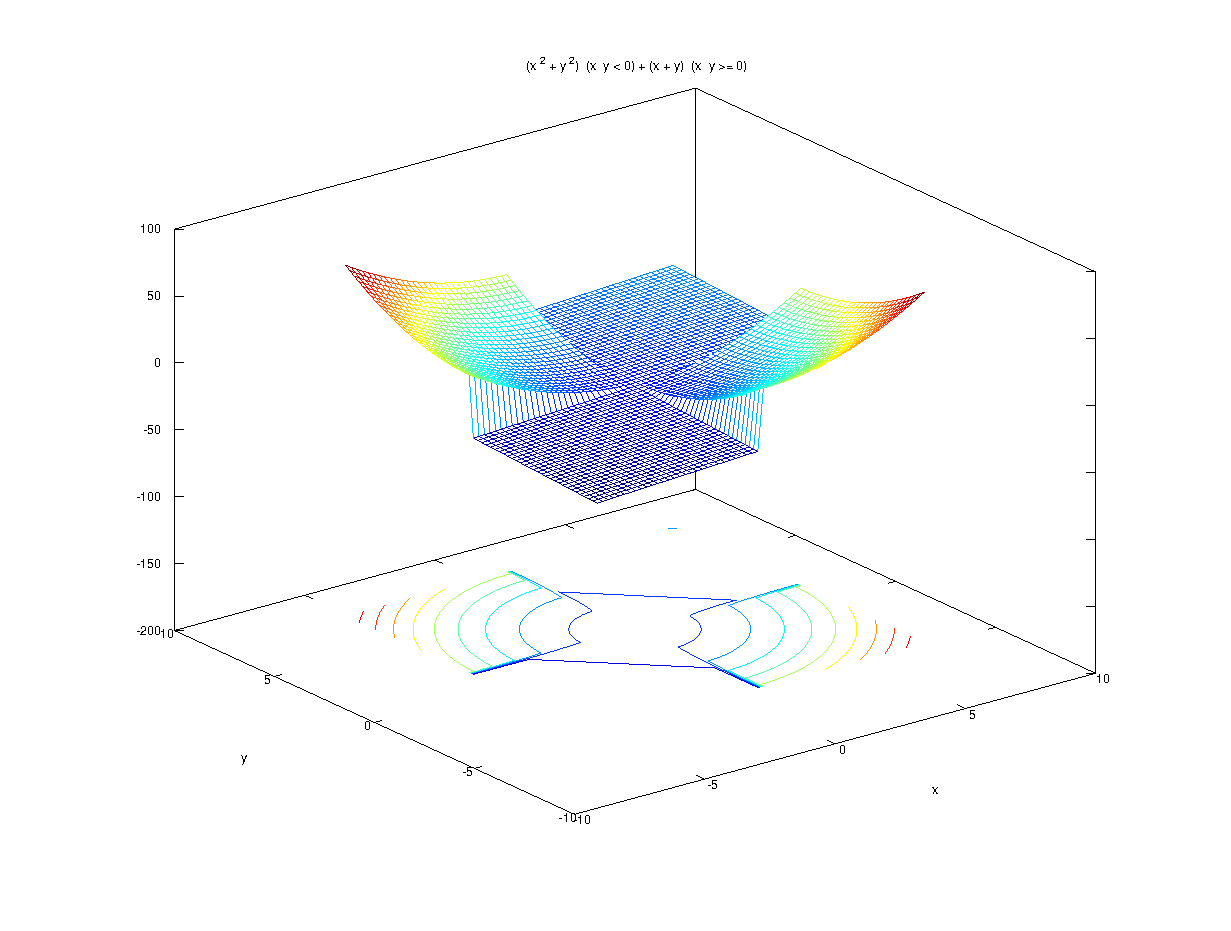
\includegraphics[width=\linewidth]{nondiff}
  \[ f(x,y) = \begin{cases} x^2+y^2 & \text{ if } xy < 0 \\
    x + y \text{ if } xy \geq 0 
  \end{cases}
  \]
\end{frame}

\begin{frame}
  \frametitle{Total derivative}
  \begin{definition}
    Let $f: \R^n \to \R$. The \textbf{derivative} (or total derivative
    or differential) of $f$ at $x_0$ is a linear mapping, $Df_{x_0}:
    \R^n \to \R^1$ such that
    \begin{align*}
      \lim_{h \to 0} \frac{\left|f(x_0 + h) - f(x_0) - Df_{x_0} h\right|} {\norm{h}}
      = 0.
    \end{align*}
  \end{definition}
\end{frame}

\begin{frame}
  \begin{theorem}\label{thm:tdiff}
    Let $f: \R^n \to \R$ be differentiable at $x_0$, then
    $\frac{\partial f}{\partial x_i}(x_0)$ exists for each $i$ and 
    \[ Df_{x_0} h = 
    \begin{pmatrix} 
      \frac{ \partial f}{\partial x_1}(x_0) &
      \cdots \frac{ \partial f}{\partial x_n }(x_0)
    \end{pmatrix} h. \]
  \end{theorem}
\end{frame}

\begin{frame}[shrink]
  \begin{proof}
    The definition of derivative says that
    \begin{align*}
      \lim_{t \to 0} \frac{\left|f(x_0 + e_i t) - f(x_0) - Df_{x_0} (e_i t)\right|}
      {\norm{e_i t} } & = 0 \\
      \lim_{t \to 0} \frac{f(x_0 + e_i t) - f(x_0) - t D f_{x_0} e_i}
      {|t| } & =  0
    \end{align*}
    This implies that
    \begin{align*}
      f(x_0 + e_i t) - f(x_0) = t D f_{x_0} e_i + r_i(x_0,t)
    \end{align*}
    with $\lim_{t \to 0} \frac{|r_i(x_0,t)|}{|t|} = 0$. Dividing by $t$, 
    \begin{align*}
      \frac{f(x_0 + e_i t) - f(x_0)}{t} = D f_{x_0} e_i + \frac{r_i(x_0,t)}{t}
    \end{align*}
    and taking the limit
    \begin{align*}
      \lim_{t \to 0} \frac{f(x_0 + e_i t) - f(x_0)}{t} = D f_{x_0} e_i 
    \end{align*}
  \end{proof}
\end{frame}

\begin{frame}
  \begin{theorem}\label{thm:ptdiff}
    Let $f:\R^n \to \R$ and suppose its partial derivatives exist and
    are continuous in $N_\delta(x_0)$ for some $\delta>0$. Then $f$
    is differentiable at $x_0$ with 
    \[ 
    Df_{x_0}= 
    \begin{pmatrix} 
      \frac{ \partial f}{\partial x_1}(x_0) &
      \cdots \frac{ \partial f}{\partial x_n }(x_0)
    \end{pmatrix}. 
    \]
  \end{theorem}
  
  \begin{corollary}
    $f:\R^n \to \R$ has a continuous derivative on an open set $U
    \subseteq \R^n$ if and only if its partial derivatives are
    continuous on $U$
  \end{corollary}  
\end{frame}

\subsection{Mean value theorem}

\begin{frame}
  \frametitle{Mean value theorem}
  \begin{theorem}[mean value]\label{thm:mvt}
    Let $f:\R^n \to \R^1$ be in $C^1(U)$ for some open $U$. Let $x, y
    \in U$ be such that the line connecting $x$ and $y$, $\ell(x,y) =
    \{z\in \R^n: z = \lambda x + (1-\lambda) y, \lambda \in [0,1]\}$, is
    also in $U$. Then there is some $\bar{x} \in \ell(x,y)$ such that
    \[ f(x) - f(y) = Df_{\bar{x}} (x-y). \]
  \end{theorem}
\end{frame}

\begin{frame}[allowframebreaks]
  \frametitle{Results needed to prove mean value theorem} 
  \begin{theorem}
    Let $f:\R^n \to \R$ be continuous and $K \subset \R^n$ be
    compact. Then $\exists x^* \in K$ such that $f(x^*) \geq f(x)
    \forall x \in K$. 
  \end{theorem}
    
  \begin{definition}
    Let $f: \R^n \to \R$. we say that $f$ has a local maximum at $x$ if
    $\exists \delta > 0$ such that $f(y) \leq f(x)$ for all $y \in
    N_\delta(x)$. 
  \end{definition}

  \begin{theorem}
    Let $f: \R^n \to \R$ and suppose $f$ has a local maximum at $x$ and
    is differentiable at $x$. Then $Df_x = 0$. 
  \end{theorem}
\end{frame}

\begin{frame}\frametitle{Proof of mean value theorem}
  \begin{proof}
    Let $g(z) = f(y) - f(z) + \frac{f(x) - f(y)}{x-y} (z - y)$. Note
    that $g(x) = g(y) = 0$. The set $ell(x,y)$ is closed and bounded,
    so it is compact. Hence, $g(z)$ must attain its maximum on
    $\ell(x,y)$, say at $\bar{x}$, then the previous theorem shows
    that $Dg_{\bar{x}} = 0$. Simple calculation shows that
    \[ Dg_{\bar{x}} = -Df_{\bar{x}} +  \frac{f(x) - f(y)}{x-y} = 0 \]
    so 
    \[ Df_{\bar{x}}(x-y) = f(x) - f(y). \]
  \end{proof}
\end{frame}

\subsection{Functions from $\R^n \to \R^m$}

\begin{frame}[shrink]
  \frametitle{Functions from $\R^n \to \R^m$}
  \begin{definition}
    Let $f: \R^n \to \R^m$. The \textbf{derivative} (or total derivative
    or differential) of $f$ at $x_0$ is a linear mapping, $Df_{x_0}:
    \R^n \to \R^m$ such that
    \begin{align*}
      \lim_{h \to 0} \frac{\left\Vert f(x_0 + h) - f(x_0) - Df_{x_0}
          h\right\Vert} {\norm{h}} = 0. 
    \end{align*}
  \end{definition}
  \begin{itemize}
  \item Theorems \ref{thm:tdiff} and \ref{thm:ptdiff} sill hold
  \item The total derivative of $f$ can be represented by the
    $m$ by $n$ matrix of partial derivatwives (the \textbf{Jacobian}),
    \[ Df_{x_0}  = \begin{pmatrix} \frac{\partial f_1}{\partial x_1}(x_0) &
      \cdots & \frac{\partial f_1}{\partial x_n}(x_0) \\
      \vdots & & \vdots \\
      \frac{\partial f_m}{\partial x_1}(x_0) & \cdots & \frac{\partial
        f_m}{\partial x_n}(x_0)  
    \end{pmatrix}. \] 
  \end{itemize}
\end{frame}

\begin{frame}
  \begin{corollary}[mean value for $\R^n \to \R^m$]\label{thm:mvtm}
    Let $f:\R^n \to \R^m$ be in $C^1(U)$ for some open $U$. Let $x, y
    \in U$ be such that the line connecting $x$ and $y$, $\ell(x,y) =
    \{z\in \R^n: z = \lambda x + (1-\lambda) y, \lambda \in [0,1]\}$, is
    also in $U$. Then there are $\bar{x}_j \in \ell(x,y)$ such that
    \[ f_j(x) - f_j(y) = D{f_j}_{\bar{x}_j} (x-y) \]
    and
    \[ f(x) - f(y) = \begin{pmatrix} D{f_1}_{\bar{x}_1} \\
      \vdots \\
      D{f_m}_{\bar{x}_m} \end{pmatrix} (x-y). 
    \]  
  \end{corollary}
\end{frame}

\subsection{Chain rule}

\begin{frame}\frametitle{Chain rule}
  \begin{itemize}
  \item $f(g(x)) = f'(g(x)) g'(x)$. 
  \end{itemize}
  \begin{theorem} \label{thm:chain}
    Let $f:\R^n \to \R^m$ and $g: \R^k \to \R^n$. Let $g$ be
    continuously differentiable on some open set $U$ and $f$ be
    continuously differentiable on $g(U)$. Then $h:\R^k \to \R^m$, $h
    (x) = f(g(x))$ is continuously differentiable on $U$ with 
    \[ Dh_x = D f_{g(x)} D g_x \]
  \end{theorem}
\end{frame}

\begin{frame}[shrink]
  \begin{proof}
    Let $x \in U$. Consider
    \begin{align*}
      \frac{\norm{ f(g(x+d)) - f(g(x))}} {\norm{d}}.
    \end{align*}
    Since $g$ is differentiable by the mean value theorem, $g(x+d) =
    g(x) + Dg_{\bar{x}(d)} d$, so
    \begin{align*}
      \norm{ f(g(x+d)) - f(g(x))} = &  
      \norm{ f(g(x) + D g_{\bar{x}(d)} d ) - f(g(x))} \\
      \leq & \norm{f(g(x) + D g_x d) - f(g(x))} + \epsilon
    \end{align*}
    where the inequality follows from the the continuity of $D g_x$ and
    $f$, and holds for any $\epsilon >0$. $f$ is differentiable, so
    \[ \lim_{D g_x d \to 0} \frac{\norm{f(g(x) + D g_x d) -
        f(g(x)) - D f_{g(x)} D g_x d}} {\norm{D g_x d}} = 0 \]
    Using the Cauchy-Schwarz inequality, $\norm{D g_x d} \leq \norm{D
      g_x} \norm{d}$, so
    \[ \lim_{ d \to 0} \frac{\norm{f(g(x) + D g_x d) -
        f(g(x)) - D f_{g(x)} D g_x d}} {\norm{d}} = 0. \]   
  \end{proof}
\end{frame}

\subsection{Higher order derivatives}
\begin{frame}\frametitle{Higher order derivatives}
  \begin{itemize}
  \item Take higher order derivatives of multivariate functions just
    like of univariate functions. 
  \item If $f: \R^n \to \R^m$, then is has $nm$
    partial first derivatives. Each of these has $n$ partial derivatives,
    so $f$ has $n^2m$ partial second derivatives, written
    $\frac{\partial^2 f_k}{\partial x_i \partial x_j}$. 
  \end{itemize}
\end{frame}

\begin{frame}
  \begin{theorem}
    Let $f: \R^n \to \R^m$ be twice continuously differentiable on some
    open set $U$. Then
    \[ \frac{\partial^2 f_k}{\partial x_i \partial
      x_j}(x) =  \frac{\partial^2 f_k}{\partial x_j \partial
      x_i} (x) \]
    for all $i,j,k$ and $ x \in U$.
  \end{theorem}
\end{frame}

\begin{frame}
  \begin{corollary}
    Let $f: \R^n \to \R^m$ be $k$ times continuously differentiable on
    some open set $U$. Then 
    \[ \frac{\partial^k f}{\partial x_1^{j_1} \times \cdots
      \times \partial x_n^{j_n}} = 
    \frac{\partial^k f}{\partial x_{p(1)}^{j_{p(1)}} \times \cdots \times \partial
      x_{p(n)}^{j_{p(n)}}} \]
    where $\sum_{i=1}^n j_i = k$ and $p:\{1,..,n\} \to \{1,...,n\}$ is
    any permutation (i.e. reordering).
  \end{corollary}
\end{frame}

\subsection{Taylor series}
\begin{frame}\frametitle{Taylor series}
  \begin{theorem}[Univarite Taylor series]
    Let $f: \R \to \R$ be $k+1$ times continuously differentiable on some
    open set $U$, and let $a$, $a+h \in U$. Then 
    \[ f(a+h) = f(a) + f'(a) h + \frac{f^2(a)}{2} h^2 + ... +
    \frac{f^k(a)}{k!} h^k + \frac{f^{k+1}(\bar{a})}{(k+1)!} h^{k+1} 
    \]
    where $\bar{a}$ is between $a$ and $h$. 
  \end{theorem}
\end{frame}

\begin{frame}
  \begin{theorem}[Multivariate Taylor series]
    Let $f:\R^n \to \R^m$ be $k$ times continuously differentiable on
    some open set $U$ and $a, a+h \in U$. Then there exists a $k$ times
    continuously differentiable function $r_k(a,h)$ such that
    \[ f(a+h) = f(a) + \sum_{\sum_{i=1}^n {j_i}=1}^k\frac{1}{k!}
    \frac{\partial^{\sum j_i} f}{\partial x_{1}^{j_1} \cdots \partial
      x_{n}^{j_n}}(a) h_1^{j_1}h_2^{j_2} \cdots h_n^{j_n} +
  r_k(a,h) \]
  and $\lim_{h \to 0} \norm{r_k(a,h)}{\norm{h}^k} = 0$
  \end{theorem}
\end{frame}

\begin{frame}
  \begin{proof}
    Follows from the mean value theorem. For $k=1$, the mean value
    theorem says that
    \begin{align*}
      f(a+h) - f(a) = & Df_{\bar{a}} h \\
      f(a+h) = & f(a) + Df_{\bar{a}} h \\
      = & f(a) + Df_{a} h + \underbrace{(Df_{\bar{a}} -Df_a)h}_{r_1(a,h)}  
    \end{align*}
    $Df_a$ is continuous as a function of $a$, and as $h \to 0$,
    $\bar{a} \to a$, so $\lim_{h \to 0} r_1(a,h) = 0$, and the theorem
    is true for $k = 1$. For general $k$, suppose we have proven the
    theorem up to $k-1$. Then repeating the same argument with the
    $k-1$st derivative of $f$ in place of $f$ shows that theorem is true
    for $k$. 
  \end{proof}
\end{frame}

\section{Functions on vector spaces}

\begin{frame}
  \begin{definition}
    Let $f: V \to W$. The Fr\'{e}chet \textbf{derivative} of $f$ at
    $x_0$ is a continuous\footnote{If $V$
      and $W$ are finite dimensional, then all linear functions are
      continuous. In infinite dimensions, there can be discontinuous
      linear functions.} linear mapping, $Df_{x_0}: V \to W$ such that
    \begin{align*}
      \lim_{h \to 0} \frac{\left\Vert f(x_0 + h) - f(x_0) - Df_{x_0}
          h\right\Vert} {\norm{h}} = 0. 
    \end{align*}
  \end{definition}
  \begin{itemize}
  \item Just another name for total derivative
  \end{itemize}
\end{frame}

\begin{frame}
  \begin{example}\label{ex:fre}
    Let $V = \mathcal{L}^\infty(0,1)$ and $W = \R$. Suppose $f$ is given by
    \[ f(x) = \int_0^1 g(x(\tau),(\tau)) d\tau \] 
    for some continuously differentiable function $g:\R^2 \to
    \R$. 
    Then $Df_{x}$ is a linear transformation from $V$ to $\R$. How
    can we calculate $Df_x$?  
  \end{example}
\end{frame}

\begin{frame}
  \begin{definition}
    Let $f: V \to W$, $v \in V$ and $x \in U \subseteq V$ for some open
    $U$. The \textbf{directional derivative} (or G\^{a}teaux derivative
    when $V$ is infinite dimensional)  in direction $v$ at $x$ is
    \begin{align*}
      df(x;v) = \lim_{\alpha \to 0} \frac{f(x + \alpha v) - f(x)}{\alpha}.
    \end{align*}  
    where $\alpha \in \R$ is a scalar.
  \end{definition}
\end{frame}

\begin{frame}\frametitle{Relationship between directional and total derivative}
  \begin{lemma}\label{lem:fregat}
    If $f: V \to W$ is Fr\'{e}chet differentiable at $x$, then the
    G\^{a}teaux derivative, $df(x;v)$, exists for all $v \in V$, and
    \[ df(x;v) = Df_x v. \]
  \end{lemma}

  \begin{lemma}\label{lem:gatfre}
    If $f: V \to W$ has G\^{a}teaux derivatives that are linear in $v$
    and ``continuous'' in $x$ in the sense that $\forall \epsilon>0$
    $\exists \delta > 0$ such that if $\norm{x_1 - x} < \delta$, then
    \begin{align*}
      \sup_{v \in V} \frac{\norm{df(x_1;v) - df(x;v)}}{\norm{v}} < \epsilon
    \end{align*}
    then $f$ is Fr\'{e}chet differentiable with $Df_{x_0} v = df(x;v)$.
  \end{lemma}
\end{frame}

\begin{frame}[shrink]
  \frametitle{Calculating Fr\'{e}chet derivative}
  \begin{example}
    Let $V = \mathcal{L}^\infty(0,1)$ and $W = \R$. Suppose $f$ is
    given by 
    \[ f(x) = \int_0^1 g(x(\tau),(\tau)) d\tau \] 
    \begin{itemize}
    \item Directional (G\^{a}teaux) derivatives:
      \begin{align*}
        df(x;v) = & \lim_{\alpha \to 0} \frac{\int_0^1 g(x(\tau) + \alpha
          v(\tau), \tau) d\tau}{\alpha} \\
        = & \int_0^1 \frac{\partial g}{\partial x}(x(\tau),\tau) v(\tau)
        d\tau
      \end{align*}    
    \item Check that continuous and linear in $v$
    \item Or guess and verify that
      \[ Df_x(v) = \int_0^1 \frac{\partial g}{\partial x}(x(\tau),\tau)
      v(\tau) d\tau \]
      satisfies
      \[ \lim_{h \to 0} \frac{\norm{f(x+h) - f(x) - Df_x(h)
        }}{\norm{h}} =  0 \]
    \end{itemize}      
  \end{example}  
\end{frame}

\end{document}
